% Copyright (c) 2014,2016 Casper Ti. Vecto

\chapter{相關理論與技術}
	
	\section{比特幣(Bitcoin)}

		\begin{table}[htbp]
		\centering
		\caption{比特幣簡介}
		\label{IntroductiontoBitcoin}
		\begin{tabular}{|l|l|}
		\hline
		第一個區塊生成時間 & 2009年1月3日 \\ \hline
		比特幣預計總產量 & 21,000,000 BTC \\ \hline
		比特幣目前總產量 & 16,921,800 BTC \\ \hline
		最新區塊高度 & 513743 \\ \hline
		比特幣總市值(人民幣) & 5兆 \\ \hline
		比特幣全節點的數量 & 11147 個 \\ \hline
		單日比特幣交易金額(BTC) & 124,017.02430718 BTC \\ \hline
		單日交易筆數 & 196,606 筆 \\ \hline
		比特幣區塊鏈大小 & 188.89 GB \\ \hline
		平均區塊大小 & 0.75 MB \\ \hline
		平均生成單一區塊所需時間 & 9.67 分鐘 \\ \hline
		單日產出比特幣數量 & 1,775 BTC \\ \hline
		挖礦難易度參數 & 3,290,605,988,755 \\ \hline
		全網挖礦算力 & 23,555,075.18 THash/s \\ \hline
		\end{tabular}
		\end{table}

		比特幣(Bitcoin,BTC)表\ref{IntroductiontoBitcoin}是比特幣系統的相關參數簡介,比特幣是一個點對點式的電子現金系統,集成了非對稱式金鑰密碼學(Asymmetric Key Cryptography)\supercite{AsymmetricKeyCryptography}、簽章密碼學(Signature Cryptography)\supercite{Apublickeycryptosystemandasignatureschemebasedondiscretelogarithms}、零知識證明密碼學(Zero Knowledge Proof Cryptography)\supercite{Zero-KnowledgeProofsofIdentity}、哈希函數密碼學(Hash Function Cryptography)、共識算法(Consensus Algorithm)\supercite{Anonymousbyzantineconsensusfrommoderately-hardpuzzles:Amodelforbitcoin}諸多技術建構了一個分散式、不需要仰賴中心化機構加以維護的交易帳本。在接下來的章節中將逐一進行詳盡的說明每個技術在各個環節中所扮演的角色。

		\section{比特幣地址(Bitcoin Address)}
		⽐特幣地址為⽐特幣的載體,深⼊瞭解⽐特幣的地址⽣成相關算法、⽐特幣地址⽣成過程、多重簽章,可以近⼀步應⽤在區塊鏈的實名交易監督系統。

			\subsection{比特幣地址生成相關算法}
			在點對點的現金系統中,首先必須先生成一個地址,在比特幣的協議中有著既定的程序生成地址。運用到的技術包括亂數產生器、secp256k1\supercite{johnson2001elliptic}、SHA-256(哈希函數)\supercite{DBLP:conf/fse/KhovratovichRS12}、RIPEMD-160(哈希函數)\supercite{DBLP:conf/isw/MendelPRR06}、Base58\supercite{Base58}。接下來將詳述每一個函數的運作過程以及意義,最後說明比特幣交易地址生成的每一個步驟。
			
				\subsubsection{亂數產生器(Random number generator)}
				亂數在密碼學中是個相當重要的一環,在比特幣系統中更是重要,畢竟生成的亂數會變成比特幣的私鑰,私鑰是簽署資產轉移的唯一方式,在比特幣地址中的亂數產生器會產出一個256 bits長度的亂數,也就是私鑰,256 bits的長度可以表現的組態空間為$2^{256}$,換算成十進位表示為$1.1579209x10^{77}$,要在這組態空間中,以亂數產生同樣的一把私鑰是一件困難的事,但也有國際的實驗室\supercite{TheLargeBitcoinCollider}團隊正在努力的窮舉比特幣$2^{256}$的組態空間,如圖\ref{LBC}所示,根據LBC公佈的數據顯示,目前已經完成了$2.330109x10^{16}$個地址探索。雖然$10^{16}$的級別與$10^{77}$的級別相距甚遠,但LBC已探索的組態空間中擊中了15個比特幣地址,該團隊也成功將這15 個地址下的1.180899個比特幣轉走。

				\begin{figure}[htbp]
					\centering
					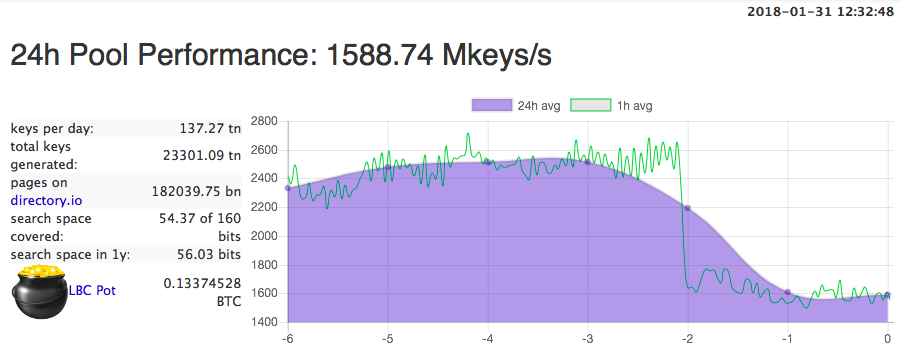
\includegraphics[width = .9\textwidth]{LBC.png}
					\caption{LBC窮舉比特幣私鑰算力狀態圖\supercite{TheLargeBitcoinCollider}}\label{LBC}
				\end{figure}

				如何建構一個亂數,在過往的亂數產生器往往會加入時間作為參數,但對於一個攻擊者而言,只需要去猜測在這段時間內目標者所有生成的可能性有極高的機率可猜出亂數。而亂數在密碼學中常會是一把私鑰的生成,在https協議中,服務器端與客戶端,建立一個加密連線的過程中也需要一個亂數去建立一個高安全性的加密通道-傳輸層安全性協定(Transport Layer Security,TLS)\supercite{dierks2008transport},在SSH協議中也採用了亂數。
		
				在過去的歷史事件中,發現Android手機版以及平板版的亂數產生器中存在著不隨機,於2013年8月比特幣開發者Mike Hearn提及“All private keys generated on Android phones/tablets are weak and some signatures have been observed to have colliding R values” \supercite{SomeSecureRandomThoughts},Bitcoin.org也發布了警告\supercite{AndroidSecurityVulnerability}簡要說明該事件的原因,以及表明影響到的比特幣錢包客戶端有Bitcoin Wallet、BitcoinSpinner、Mycelium Bitcoin Wallet、blockchain.info。這樣的錯誤源於Android本身支持的亂數產生器並不隨機,隨後Android解釋了亂數的問題並加以修正。在這Android手機亂數不夠亂的事件中,有自願者自發性地公佈自己的損失狀態,總金額為55.82152538個比特幣\supercite{Badsignaturesleading},但因為比特幣屬於被動的性質,無人主動回報即不會加入統計中,所以總損失估計會超過55.82152538個比特幣。

				\subsubsection{Secp256k1}
				在密碼學中有分對稱式加密與非對稱式加密,對稱式加密又分為信息流加密與信息塊加密,信息流加密著名的是由美國密碼學家Ron Rivest教授設計,包括RC2(1987年)\supercite{OnthedesignandsecurityofRC2}、RC4(1987年)\supercite{Rc4}、RC5(1994年)\supercite{TheRC5encryptionalgorithm}、RC6(1998年)\supercite{TheRC6blockcipher.v1.1August201998};信息塊加密著名的有數據加密標準(Data Encryption Standard,DES,1975年)\supercite{Dataencryptionstandard}、三重數據加密算法(Triple Data Encryption Algorithm,Triple DES,1998年)\supercite{TrippleDataEncryptionAlgorithmModesofOperation}、高級加密標準(Advanced Encryption Standard,AES,1998年)\supercite{ThedesignofRijndael:AES-theadvancedencryptionstandard};非對稱式加密最廣為人知的有RSA(Rivest–Shamir–Adleman,1977年)\supercite{Cryptographiccommunicationssystemandmethod}、橢圓曲線密碼學(Elliptic curve cryptography,ECC,1985年)\supercite{Ellipticcurvecryptosystems}。
				非對稱式加密與對稱式加密最大的不同在於,對稱式加密在加密解密的過程中只需要一把鑰匙,而非對稱式加密會生成兩把鑰匙分別為私鑰與公鑰,在算法的設計上一開始會以亂數產生一把私鑰,再經由非對稱式加密算法推導出公鑰,推導出的公鑰在非對稱式密碼學中並無直接的方法可以反推至私鑰,如此一來確立私鑰的安全性。非對稱式密碼的使用場景有兩種,第一種是希望收到加密信息的使用者Alice,Alice會生成私鑰存儲在自己本地端的電腦中,並將推導出的公鑰公佈在網絡上,這時希望聯繫Alice的使用者Bob在網絡上取得公鑰後,Bob會以Alice的公鑰進行加密,之後將密文寄送給Alice,在傳遞信息的過程中,即使網絡存在著監聽,也無法將信息順利解密,唯有Alice收到信息後使用Alice原本產生該公鑰的私鑰,才可以解出明文。第二種則應用在比特幣的交易之數字簽名以及交易驗證交易,比特幣地址的創建過程中會透過secp256k1生成私鑰公鑰對,在創建比特幣交易的過程中,使用該地址的私鑰對該地址未花費的輸出(Unspent Transaction Output,UTXO)進行數字簽名,完成數字簽名後會與公鑰以及交易信息一起廣播到比特幣網絡的交易緩存池當中,比特幣交易緩存池存在於所有比特幣全節點當中,主要存儲所有未被收入到比特幣區塊鏈內的所有交易,也就是零確認交易,等待礦工將該筆交易收入至比特幣區塊鏈當中。
				比特幣採用的secp256k1是屬於橢圓曲線密碼學中的一個版本,不同的橢圓曲線版本的差異在於不同的初始參數,包括橢圓曲線方程$$y^2=x^3+ax+b$$、$p$=FFFFFFFFFFFFFFFFFFFFFFFFFFFFFFFFFFFFFFFFFFFFFFFFFFFFFFFEFFFFFC2F為巨大的素數、G點被稱爲⽣成點的常數點亦稱為基點。至於為什麼選擇ECC而非RSA的主要原因,其一在於ECC在生成密鑰對所需的時間更佳快速,圖\ref{ECCtime}為Nicholas Jansma於2004年針對ECC與RSA的密鑰對生成時間與數字簽名所需時間的論文\supercite{Performancecomparisonofellipticcurveandrsadigitalsignatures}顯示,當ECC產生571 bits的密鑰長度,RSA要達到相同的安全性需要生成15360 bits,這也導致生成時間產生高達471倍之差距。
				
				\begin{figure}[htbp]
					\centering
					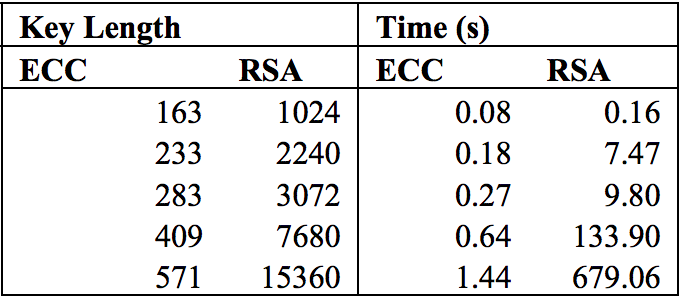
\includegraphics[width = .5\textwidth]{ECCtime.png}
					\caption{ECC與RSA的密鑰對生成時間比較圖\supercite{Performancecomparisonofellipticcurveandrsadigitalsignatures}}\label{ECCtime}
				\end{figure}

				除了在密鑰對生成時間ECC有著比RSA更高效的算法外,在安全性上ECC可以更短的密鑰長度達到與RSA相同的安全強度,L Ducas針對ECC、RSA、BLISS\supercite{LatticesignaturesandbimodalGaussians}做出了深度的安全性探討\supercite{LatticesignaturesandbimodalGaussians},圖\ref{LatticesignaturesandbimodalGaussians}同樣達到80 bits的安全性級數,RSA 1024需要1024 bits,ECDSA 160\supercite{DeploymentsofEllipticCurveCryptography}僅需要160 bits,該篇論文除了探討RSA與ECDSA之外,更大的部分在闡述量子計算機對於既有的傳統密碼帶來的抨擊,有機會快速窮舉$2^{256}$的比特幣私鑰,在未來量子計算機的蓬勃發展擁有2000 qbits運算能力,量子計算機可以快速窮舉破解所有的比特幣私鑰。因此發展針對量子計算機設計的數字簽名算法成為密碼學上嶄新的議題,而BLISS則為針對量子計算機所設計的抗量子計算的簽章算法。

				\begin{figure}[htbp]
					\centering
					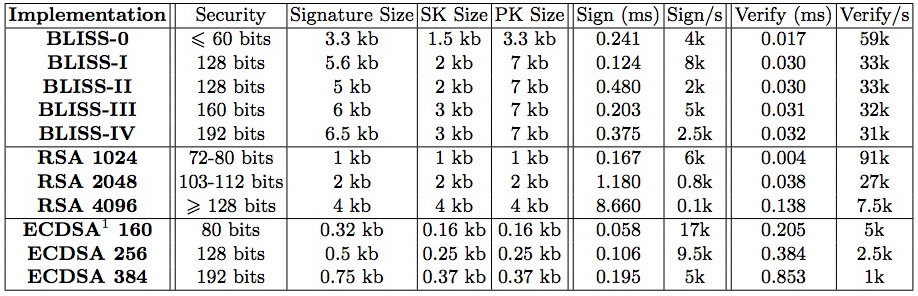
\includegraphics[width = 1\textwidth]{LatticesignaturesandbimodalGaussians.png}
					\caption{算法BLISS、RSA、ECDSA安全級數比較圖\supercite{LatticesignaturesandbimodalGaussians}}\label{LatticesignaturesandbimodalGaussians}
				\end{figure}

				\subsubsection{哈希算法 SHA-256}
				SHA-256是SHA(Secure Hash Algorithm,FIPS 182-2)\supercite{DBLP:conf/fse/KhovratovichRS12}哈希算法的家族之一。SHA家族當中有著四大分支,分別為SHA-0、SHA-1、SHA-2和SHA-3,如表\ref{hashtable}所示。各種哈希算法的差異在於運算初始變數、算法所採用的運算子、接受的信息長度以及迴圈樹的不同。上述的參數差異皆由聯邦資訊處理標準(Federal Information Processing Standards,FIPS)中定義。表\ref{hashtable}中MD5不為SHA家族成員之一,但MD5為最早被廣泛使用的哈希算法,因此作為借鑒的標準。SHA-0為SHA家族中被最早提出的架構,輸出的長度為160 bits,而SHA-1提出後並無太大的變動。
				哈希算法的主要功能在於,將信息或是檔案建立一個對一的指紋,也就是哈希值,而該指紋長度會依照算法的設計輸出的長度而略有不同,表\ref{hashtable}中顯示的輸出哈希值長度,而長度也意味著該指紋的組態空間應設的大小。倘若有著不同的輸入,但映射到了相同的指紋,則將此現象稱之為碰撞。通常在信息安全領域中,只要發現該哈希算法存在著碰撞,就會被棄用。甚至是專家們提早數年提出警告,要求提早更換該哈希算法,並更換上新制定的哈希算法做應用。哈希算法的功能包括藉由生成哈希值進行檔案校驗、工作量證明算法設計以及區塊鏈中的哈希指針。
				\begin{enumerate}
				\item 生成哈希值進行檔案校驗:哈希值在過往的應用中,往往作為檔案完整性的校驗,軟件供應者會在網站中提供各式不同算法的哈希值供給使用者下載完軟件之後,使用者將檔案輸入哈希算法中生成出哈希值後進行比對。但倘若該哈希算法存在碰撞的發生,這會使得不同的檔案存在著同樣的哈希值。這也意味著軟體提供平台所提供的軟體可能存在著摻入惡意代碼後,還能生成同樣的哈希指紋,失去了檔案完整性的校驗的功能,這便成為信息安全中的重大漏洞,因此在表\ref{hashtable}中的MD5、SHA-0以及SHA-1皆為已經棄用之算法。
				\item 工作量證明算法設計:起出工作量證明算法的概念為設計一個求解困難,但驗算的過程中卻相當簡單快速。如對一個大數做因式分解是一個相當困難的事,但要驗算其結果僅需要將所有的解相乘確認是否為該大數即可證明。同樣的理念在比特幣系統中是以hash-puzzle的方式實現,hash-puzzle是利用哈希函數有著不可預期的特性,不可預期指的是假設輸入連續性的數值$1$到$n$進入到哈希函數生成哈希值,而生成的哈希值無法觀察出關聯性,可說是完全不相關的數值,且無法預期下個輸入的哈希值輸出。
				比特幣系統中的困難度變數,在hash-puzzle中定義了何謂真正的答案。在SHA-256當中輸出的值為256 bits的哈希值,困難度變數則規定了在這256bit當中,自最左邊起必須為零的位數的門檻,而在困難度變數要求必須為零的位數變多,則意味著要在連續性的數值$1$到$n$的hash-puzzle中,符合門檻的解越少。在hash-puzzle中,求得一個符合困難度變數的哈希值是困難的,但要驗算求得的觧是否符合困難度的門檻相當快速,這符合起出工作量證明算法的概念。
				\item 區塊鏈中的哈希指針:比特幣區塊鏈的區塊頭當中,當前區塊存儲著前區塊頭的雙重哈希的哈希值。當前區塊則會如資料結構鏈結串列一樣,直到鏈結到第一個比特幣區塊創世區塊,區塊鏈中的哈希指針將區塊鏈結在一起,也就形成了比特幣區塊鏈的基礎。在比特幣挖礦的過程中,礦工參與著最新區塊的hash-puzzle的解題,尋找一個符合困難度變數的輸入。但hash-puzzle 的工作證明當中觧可能不只一個,但只要符合困難度變數的觧都可以創建一個新的區塊,屆時就會在當前的區塊上同時產生分岔,分岔的區塊在彼特幣系統中皆為有效,但經過多個區塊的疊加之後,變可以抉擇出最長的鏈,該最長鏈則成為主鏈,而其他的分岔鏈,則成為孤兒塊被丟棄,當中曾記載的交易信息無效,造成該分岔鏈的交易信息回溯。比特幣區塊鏈的分岔好發於最新的區塊,如圖\ref{6confirm}所示,而越舊的區塊則越不易發生,所以在比特幣交易中默認該筆交易要在六個區塊確認後,該公司才會承認該筆交易有效。
				\end{enumerate}

				\begin{figure}[htbp]
					\centering
					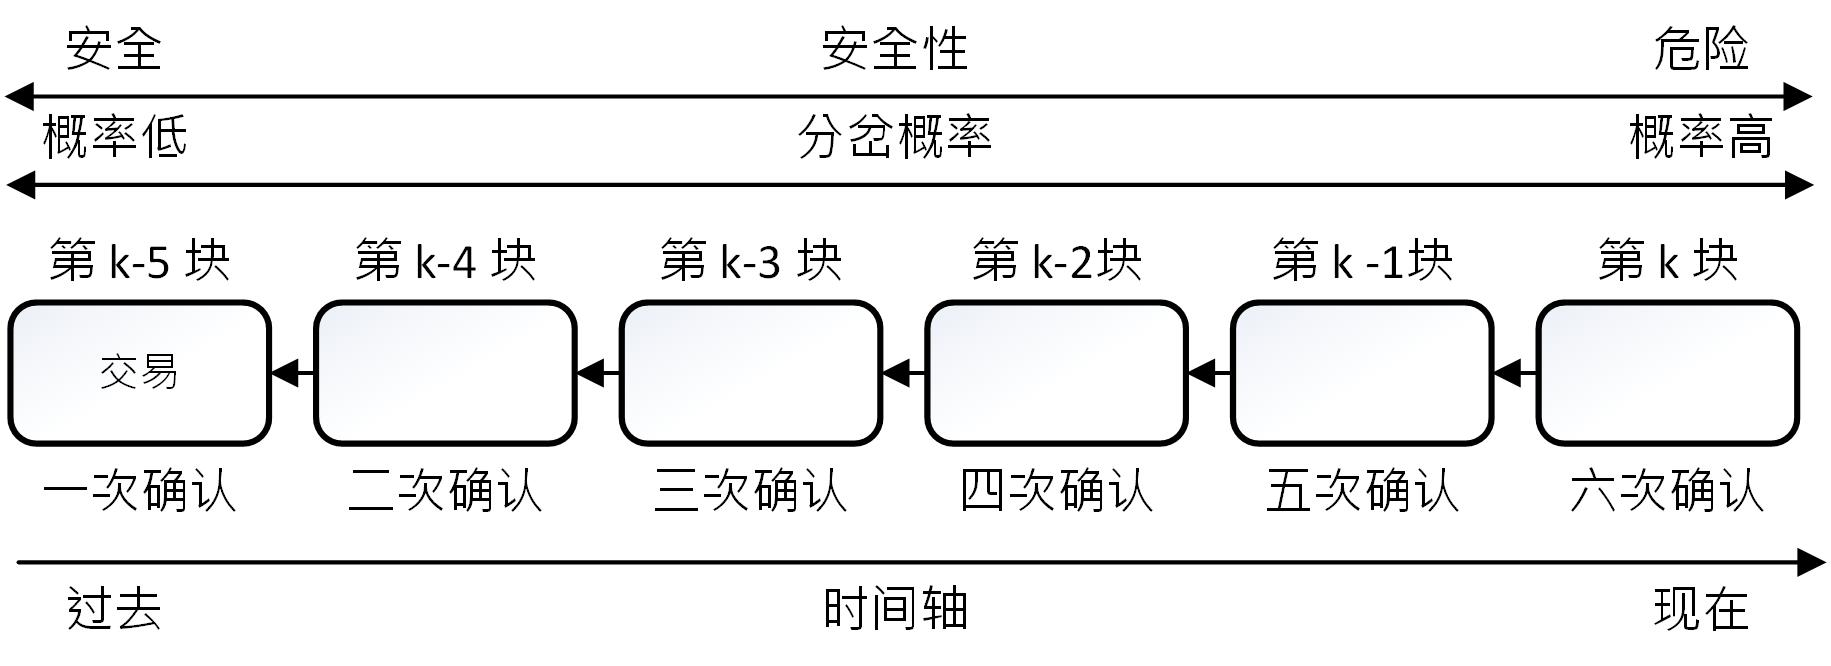
\includegraphics[width = 1\textwidth]{6confirm.jpg}
					\caption{區塊疊加示意圖}\label{6confirm}
				\end{figure}

					\begin{table}[htbp]
					\centering
					\caption{MD5、SHA-0、SHA-1、SHA-2和SHA-3比較表}
					\label{hashtable}
					\begin{tabular}{|c|c|c|c|c|c|c|}
					\hline
					算法 & 分支 & \begin{tabular}[c]{@{}c@{}}輸出\\ 哈希值\\ 長度\\ (bits)\end{tabular} & \begin{tabular}[c]{@{}c@{}}最大輸入\\ 信息長度\\ (bits)\end{tabular} & \begin{tabular}[c]{@{}c@{}}迴圈\\ 次數\end{tabular} & 使用到的運算子 & \begin{tabular}[c]{@{}c@{}}碰撞\\ 攻击\\ (bits)\end{tabular} \\ \hline
					\begin{tabular}[c]{@{}c@{}}MD5\\ 参考\end{tabular} & - & 128 & $\infty$ & 64 & \multirow{3}{*}{\begin{tabular}[c]{@{}c@{}}And, Xor, Rot, Or, \\ Add (mod $2^{32}$)\end{tabular}} & \begin{tabular}[c]{@{}c@{}}$<64$ \\ 已碰撞\end{tabular} \\ \cline{1-5} \cline{7-7} 
					SHA-0 & - & \multirow{2}{*}{160} & \multirow{2}{*}{$2^{64}-1$} & \multirow{2}{*}{80} &  & \begin{tabular}[c]{@{}c@{}}$<80$ \\ 已碰撞\end{tabular} \\ \cline{1-2} \cline{7-7} 
					SHA-1 & - &  &  &  &  & \begin{tabular}[c]{@{}c@{}}$<80$ \\ 已碰撞\end{tabular} \\ \hline
					\multirow{4}{*}{SHA-2} & SHA-224 & 224 & \multirow{2}{*}{$2^{64}-1$} & \multirow{2}{*}{64} & \multirow{2}{*}{\begin{tabular}[c]{@{}c@{}}And, Xor, Rot, Or, Shr, \\ Add (mod $2^{32}$)\end{tabular}} & 112 \\ \cline{2-3} \cline{7-7} 
					 & SHA-256 & 256 &  &  &  & 128 \\ \cline{2-7} 
					 & SHA-384 & 384 & \multirow{2}{*}{$2^{128}-1$} & \multirow{2}{*}{80} & \multirow{2}{*}{\begin{tabular}[c]{@{}c@{}}And, Xor, Rot, Or, Shr, \\ Add (mod $2^{64}$)\end{tabular}} & 192 \\ \cline{2-3} \cline{7-7} 
					 & SHA-512 & 512 &  &  &  & 256 \\ \hline
					\multirow{4}{*}{SHA-3} & SHA3-224 & 224 & \multirow{4}{*}{$\infty$} & \multirow{4}{*}{24} & \multirow{4}{*}{And, Xor, Rot, Not} & 112 \\ \cline{2-3} \cline{7-7} 
					 & SHA3-256 & 256 &  &  &  & 128 \\ \cline{2-3} \cline{7-7} 
					 & SHA3-384 & 384 &  &  &  & 192 \\ \cline{2-3} \cline{7-7} 
					 & SHA3-512 & 512 &  &  &  & 256 \\ \hline
					\end{tabular}
					\end{table}

	%			\subsubsection{RIPEMD-160}
				\subsubsection{Base58}

	%
			\subsection{比特幣地址生成過程}

			\begin{figure}[htbp]
					\centering
					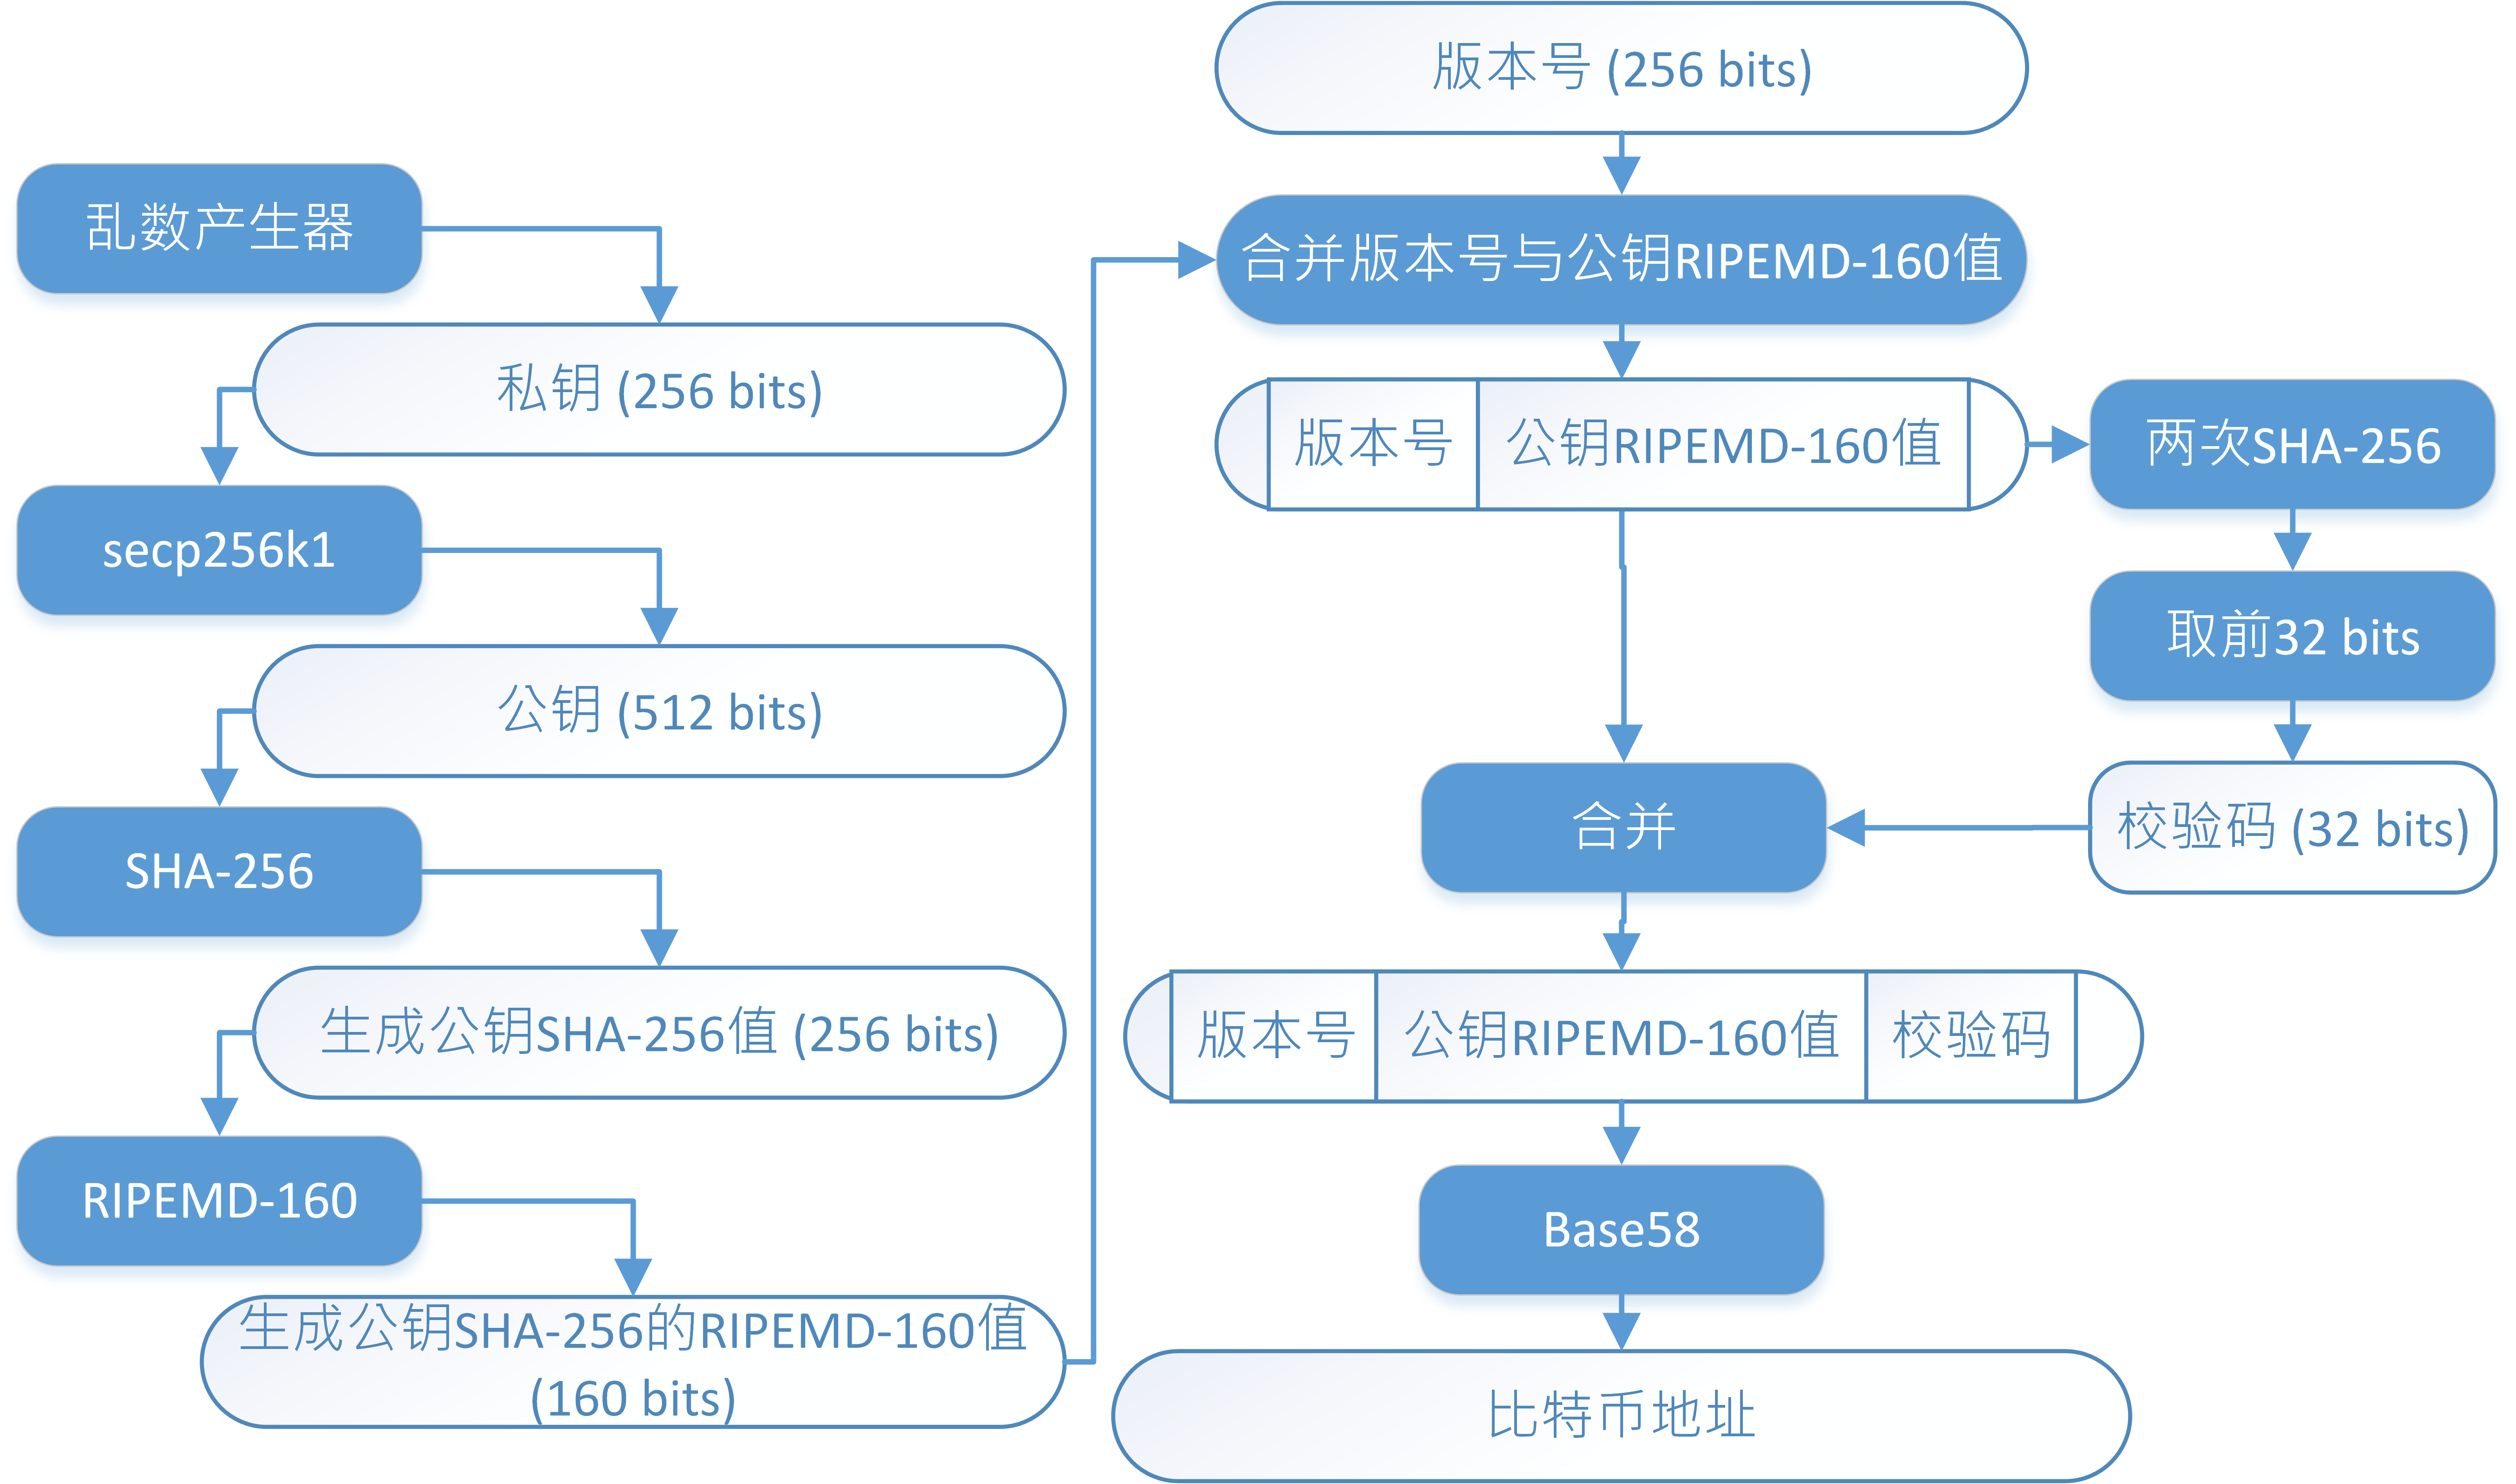
\includegraphics[width = .9\textwidth]{address.png}
					\caption{比特幣地址生成流程圖}\label{address}
			\end{figure}

			\begin{enumerate}
				\item 生成私鑰:使用亂數產生器產生一個長度為256 bits的亂數,而此亂數即成為該比特幣地址的私鑰。在比特幣的系統當中,私鑰可以透過橢圓曲線簽章算法secp256k1簽名一筆交易,廣播治比特幣網路當中。因為私鑰為該地址資金轉移的關鍵,黑客攻擊的對象皆會聚焦在比特幣私鑰,因此私鑰的保存成為比特幣系統中最為熱門的課題之一。
				\item 生成公鑰:在以亂數產生器生成私鑰之後,接下來將運用到非對稱是密碼學中的私鑰公鑰轉換算法,於比特幣系統中採用的是secp256k1
				,secp256k1是橢圓曲線密碼學中的其中一個版本,不同的版本差異在於採用不同的變數。於比特幣地址生成的過程中,secp256k1負責將上步驟生成的私鑰透過橢圓曲線算法計算出公鑰,生成的公鑰長度為512 bits,比前步驟256 bits的私鑰多了一倍的長度。在比特幣交易中,私鑰可以簽署一筆交易,在簽署完之後便會將公鑰、簽名以及交易信息廣播至比特幣網路當中等待被收入到比特幣區塊鏈當中,此時該筆交易準備被存儲在比特幣交易緩存持當中,屆時可以使用secp256k1算法對透過公鑰、簽名以及交易信息進行驗算,倘若計算出的值為真則為有效,則會讓該筆交易繼續待在交易緩存持當中,等待被收入區塊鏈內。
				\item 生成公鑰SHA-256:SHA-256為SHA家族之一,也是哈希算法的一種,因此符合哈希算法的特徵包括雪崩效應、不可預測、不可逆(單向性)以及校驗檔案是否完整性的諸多特性。在該步驟將前步驟生成長度為512 bits的公鑰作為SHA-256的輸入,產出長度僅為公鑰長度的一半的公鑰SHA-256哈希值。算該步驟使得知道公鑰SHA-256的攻擊者,更加難以用窮舉攻擊推導出該地址的公鑰。
				\item 生成公鑰SHA-256的RIPEMD-160:RIPEMD-160也是哈希算法的一種,特色與哈希算法的特徵相同,RIPEMD-160與SHA-256較為不同的部分在於RIPEMD-160生成的哈希值長度為160 bits。在前步驟中,對公鑰進行SHA-256計算,公鑰已經有了第一層的保護,而在該步驟中,再次透過RIPEMD-160取得哈希值,這使得攻擊者既使取得比特幣地址,必須針對RIPEMD-160進行破譯,再進一步對SHA-256才有機會取得該地址的公鑰,也因為這樣的設計,對於僅收取比特幣不曾花費比特幣的比特幣地址,於黑客攻擊上造成相當大的難度。
				\item 取得版本號:在比特幣系統初始的設計中,已經定義了些不同功能的比特幣地址,這些特殊功能的比特幣地址有著特殊的版本號,最為常見的為以"1"為頭的比特幣地址,該地址為比特幣系統中最早被使用且最為普遍的地址版本,該地址為一把私鑰進行比特幣地址推倒,所以僅需要一把鑰匙就可以移動該地址下的比特幣資產;第二種是以"3"為地址開頭的比特幣地址,該地址採用多重簽章技術,該技術為後續經過多項BIP才完成落實於比特幣系統當中,該地址生成的過程中,。,在第五個步驟中會加入版本號加以區分不同的地址。
				\item 校驗碼生成:校驗碼為比特幣地址生成過程中重要的一環,可在支付比特幣的過程中降低因為手誤而將比特幣轉入到不存在(不符合比特幣地址生成規則)地址的可能性。對公鑰SHA-256的RIPEMD-160再做兩次SHA-256,取該哈希值前32 bits的值作為校驗碼。
				\item 版本號、公鑰SHA-256的RIPEMD-160和校驗碼合併:版本號、第四個步驟的產生之公鑰RIPEMD-160及第五個步驟產生之校驗碼合併。
				\item 合併的結果以Base58編碼:將第六步驟組進行合併組合的結果,利用Base58進行編碼,Base58修改自Base64,其與Base64最大不同之處在於移除了"0"、"O"、"I"、"l"、"+"、"/"的字符,可以降低人工在判讀地址的錯誤率。
			\end{enumerate}

			\subsection{多重簽章(Multi-Signature)}
			% 	\subsubsection{多重簽名地址}
			 	\subsubsection{Green Address}
			 	比特幣區塊鏈技術,雖然已經利用工作量證明的方式解決了雙重支付(Double-spending)問題\supercite{Informationpropagationinthebitcoinnetwork}\supercite{Double-spendingfastpaymentsinbitcoin},但工作量證明的算法所設定之題目困難度會直接影響到每一個比特幣區塊的產出時間,這個比特幣區塊的產出時間也考慮到比特幣全節點於全世界各地的網絡同步狀況,倘若今天的區塊生成時間過短會造成全世界的比特幣節點之區塊數據不一致,這樣的數據不一致將導致比特幣區塊鏈出現分岔,在更嚴重一點甚至會造成比特幣網絡的瓦解。

			 	雙重支付問題存在於比特幣交易在未被區塊鏈確認收入到區塊鏈之前,都有機會受到惡意的攻擊者雙重支付同一筆款項。現今的比特幣區塊產出速度為十分鐘一塊,即便附上足夠的手續費也須等待將近十分鐘的時間,倘若是在手續費不足的情況下,該筆比特幣交易甚至會在比特幣交易緩存池中滯留一週的時間。在手續費足夠的情況下,十分鐘的確認時間會對實體店面的小額交易處理非常的不友善,為了在既有的比特幣區塊鏈的框架底下能夠提升交易速度,因此Green Address技術致力於在一開始創建交易的同時管控雙重支付交易的發生,他們採用了2-of-2多重簽章,也就是創建一個特殊的比特幣地址,這個比特幣地址的持有人有兩個代表人,分別為使用者與Green Address機構節點,這筆交易的建立必須要雙方同時簽署交易才被允許廣播至比特幣網絡中。若是遇到交易塞車,且節點緩存池空間不足的問題時,比特幣節點會優先遺棄手續費最低的交易,視同該筆交易不曾存在過,故若真的遇到交易被遺棄的情況,Green Address機構節點也會透內部的數據庫記錄再次廣播此筆交易,並確保此筆交易可以被收入至區塊內。Green Address機構節點也就成為了交易創建的把關者,過濾所有的雙重支付攻擊的發生,也避免交易因為比特幣網絡塞車而交易被礦工遺棄的情形。
			 	在這樣的機制下,只要是用Green Address錢包交易即可確認雙重支付攻擊是不會發生的,對商家或是收款人而言,可以得到在即時交易中不被雙重支付攻擊的保障,提升在未進入區塊鏈的交易可確定性,進而創造出即時交易的可行性。

			 	\paragraph{Green Address錢包生成過程}
			 	此節將詳細闡述Green Address錢包生成過程的重要步驟,如圖\ref{gabuild}所示。
			 	\begin{figure}[htbp]
					\centering
					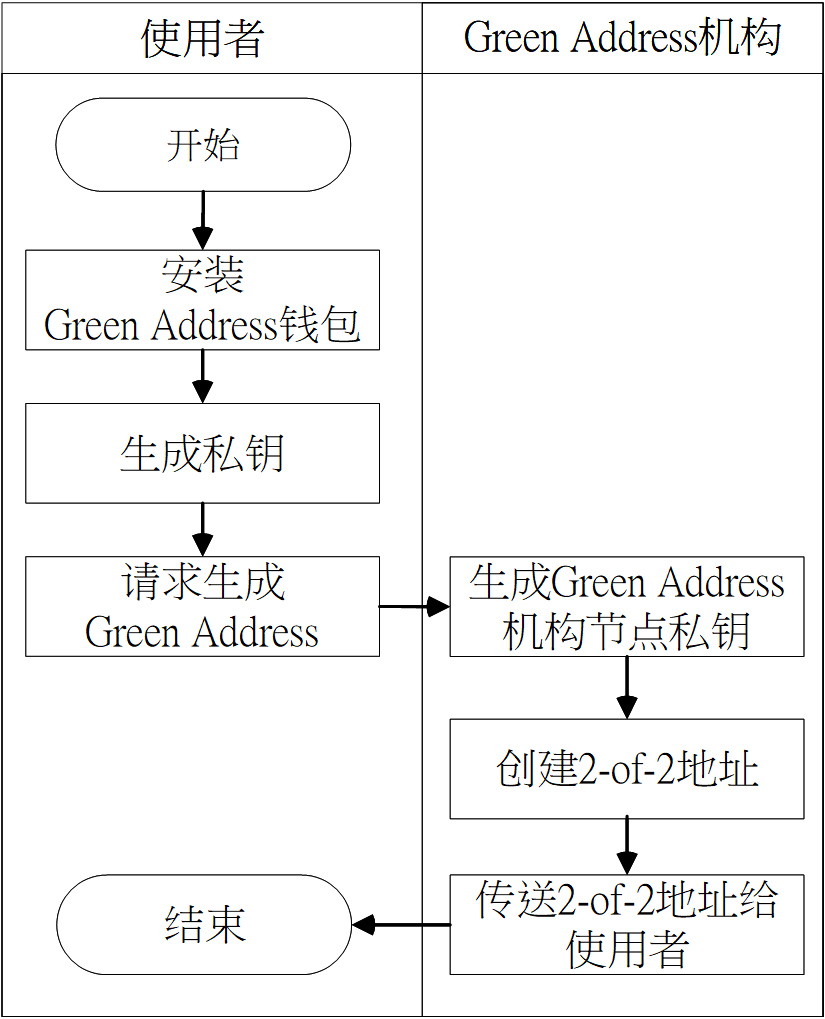
\includegraphics[width = .5\textwidth]{gabuild.png}
					\caption{Green Address錢包生成流程圖}\label{gabuild}
				\end{figure}

			 	\begin{enumerate}
			 		\item 使用者安裝Green Address比特幣錢包,並向Green Address機構節點請求創建2-of-2多重簽章比特幣地址。
			 		\item 使用者與Green Address機構節點分別生成兩把私鑰,共同創建Green Address比特幣地址。
			 		\item 當交易發起時,使用者使用自己的私鑰簽署該筆交易。
			 		\item 將該筆交易傳送到Green Address機構節點。
			 		\item Green Address機構節點收到後,檢查該筆交易是否存在雙重支付攻擊。
			 		\item 確認無攻擊跡象後便廣播至比特幣網絡中。
			 	\end{enumerate}

			 	\paragraph{Green Address交易發起流程}
			 	說明完Green Address地址是如何創建之後,本節將詳細說明如何運用多重簽章地址發起交易至比特幣網絡中,如圖\ref{gatx}所示。

			 	\begin{figure}[htbp]
					\centering
					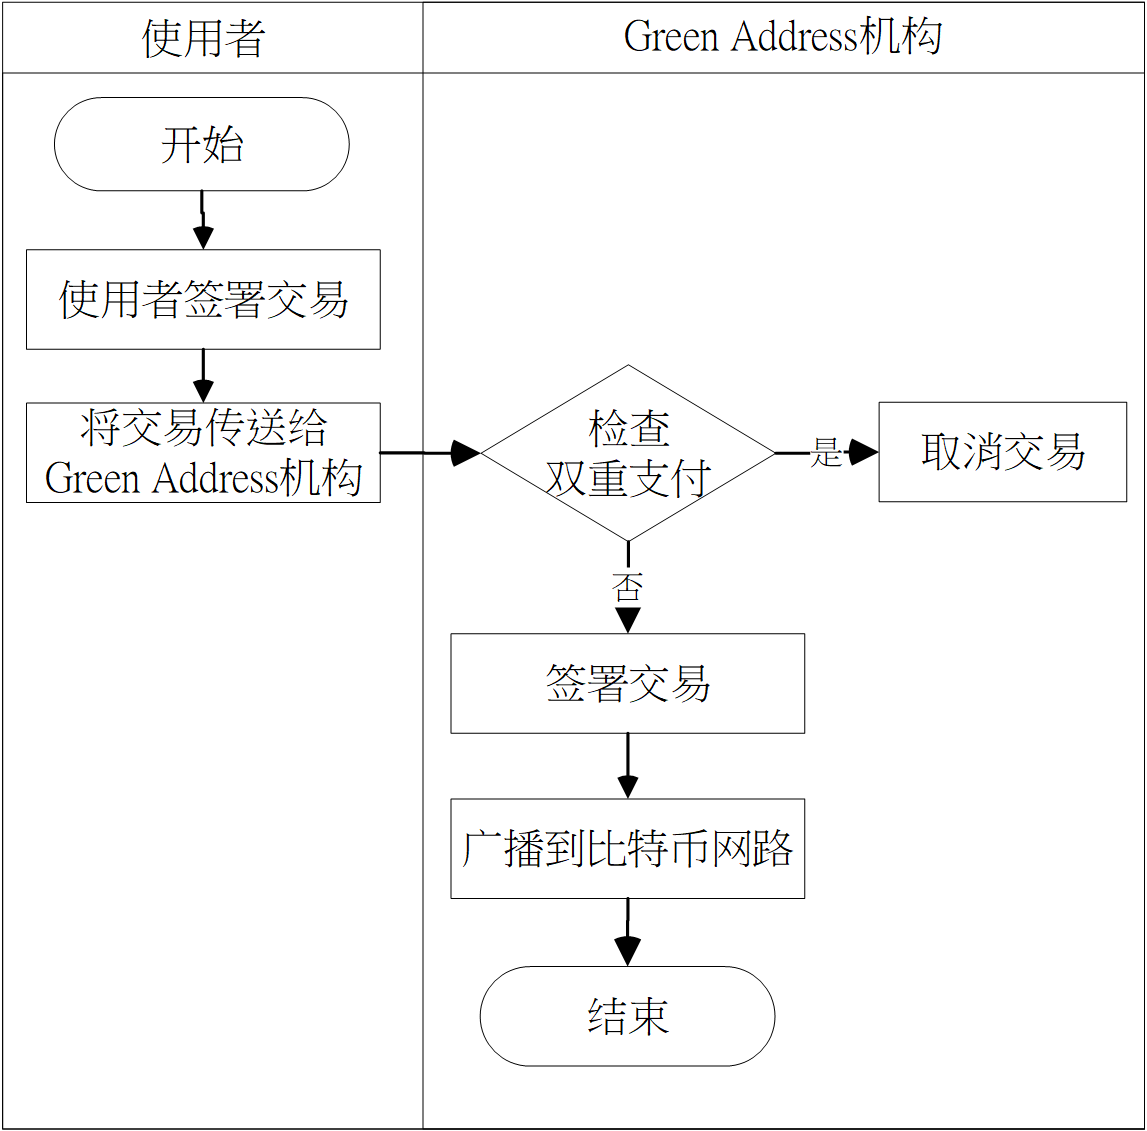
\includegraphics[width = .7\textwidth]{gatx.png}
					\caption{Green Address交易發起流程圖}\label{gatx}
				\end{figure}

				\begin{enumerate}
					\item 使用者使用原本創建Green Address的私鑰,並完成簽署交易。
					\item 因為是多重簽章地址,所以該交易需傳送至Green Address機構節點。
					\item Green Address機構節點收到交易信息後檢查該交易的發起地址是否存在雙重支付,倘若有雙重支付則遺棄;若無雙重支付則往下一個步驟。
					\item Green Address機構以Green Address的私鑰簽署該筆交易。
					\item 將該筆交易封包廣播至比特幣網絡。
				\end{enumerate}

		\section{區塊鏈(Blockchain)}
		%區塊頭所有的結構
		自2009年以來,加密貨幣比特幣的誕生引發了新的貨幣革命浪潮,基於密碼學,點對點網絡,共識算法和區塊鏈技術,它們被結合成比特幣等加密貨幣。到目前為止,它在九年內發生大量的襲擊和欺詐事件後仍然在積極努力。 比特幣一直是互聯網上最具代表性的加密貨幣,同時是區塊鏈技術最重要的應用之一,以下我們將描述區塊鏈技術的一些細節。

			%%%%%%\subsection{本區塊大小的值 }
			\subsection{區塊頭(Block Header)}

			\begin{figure}[htbp]
				\centering
				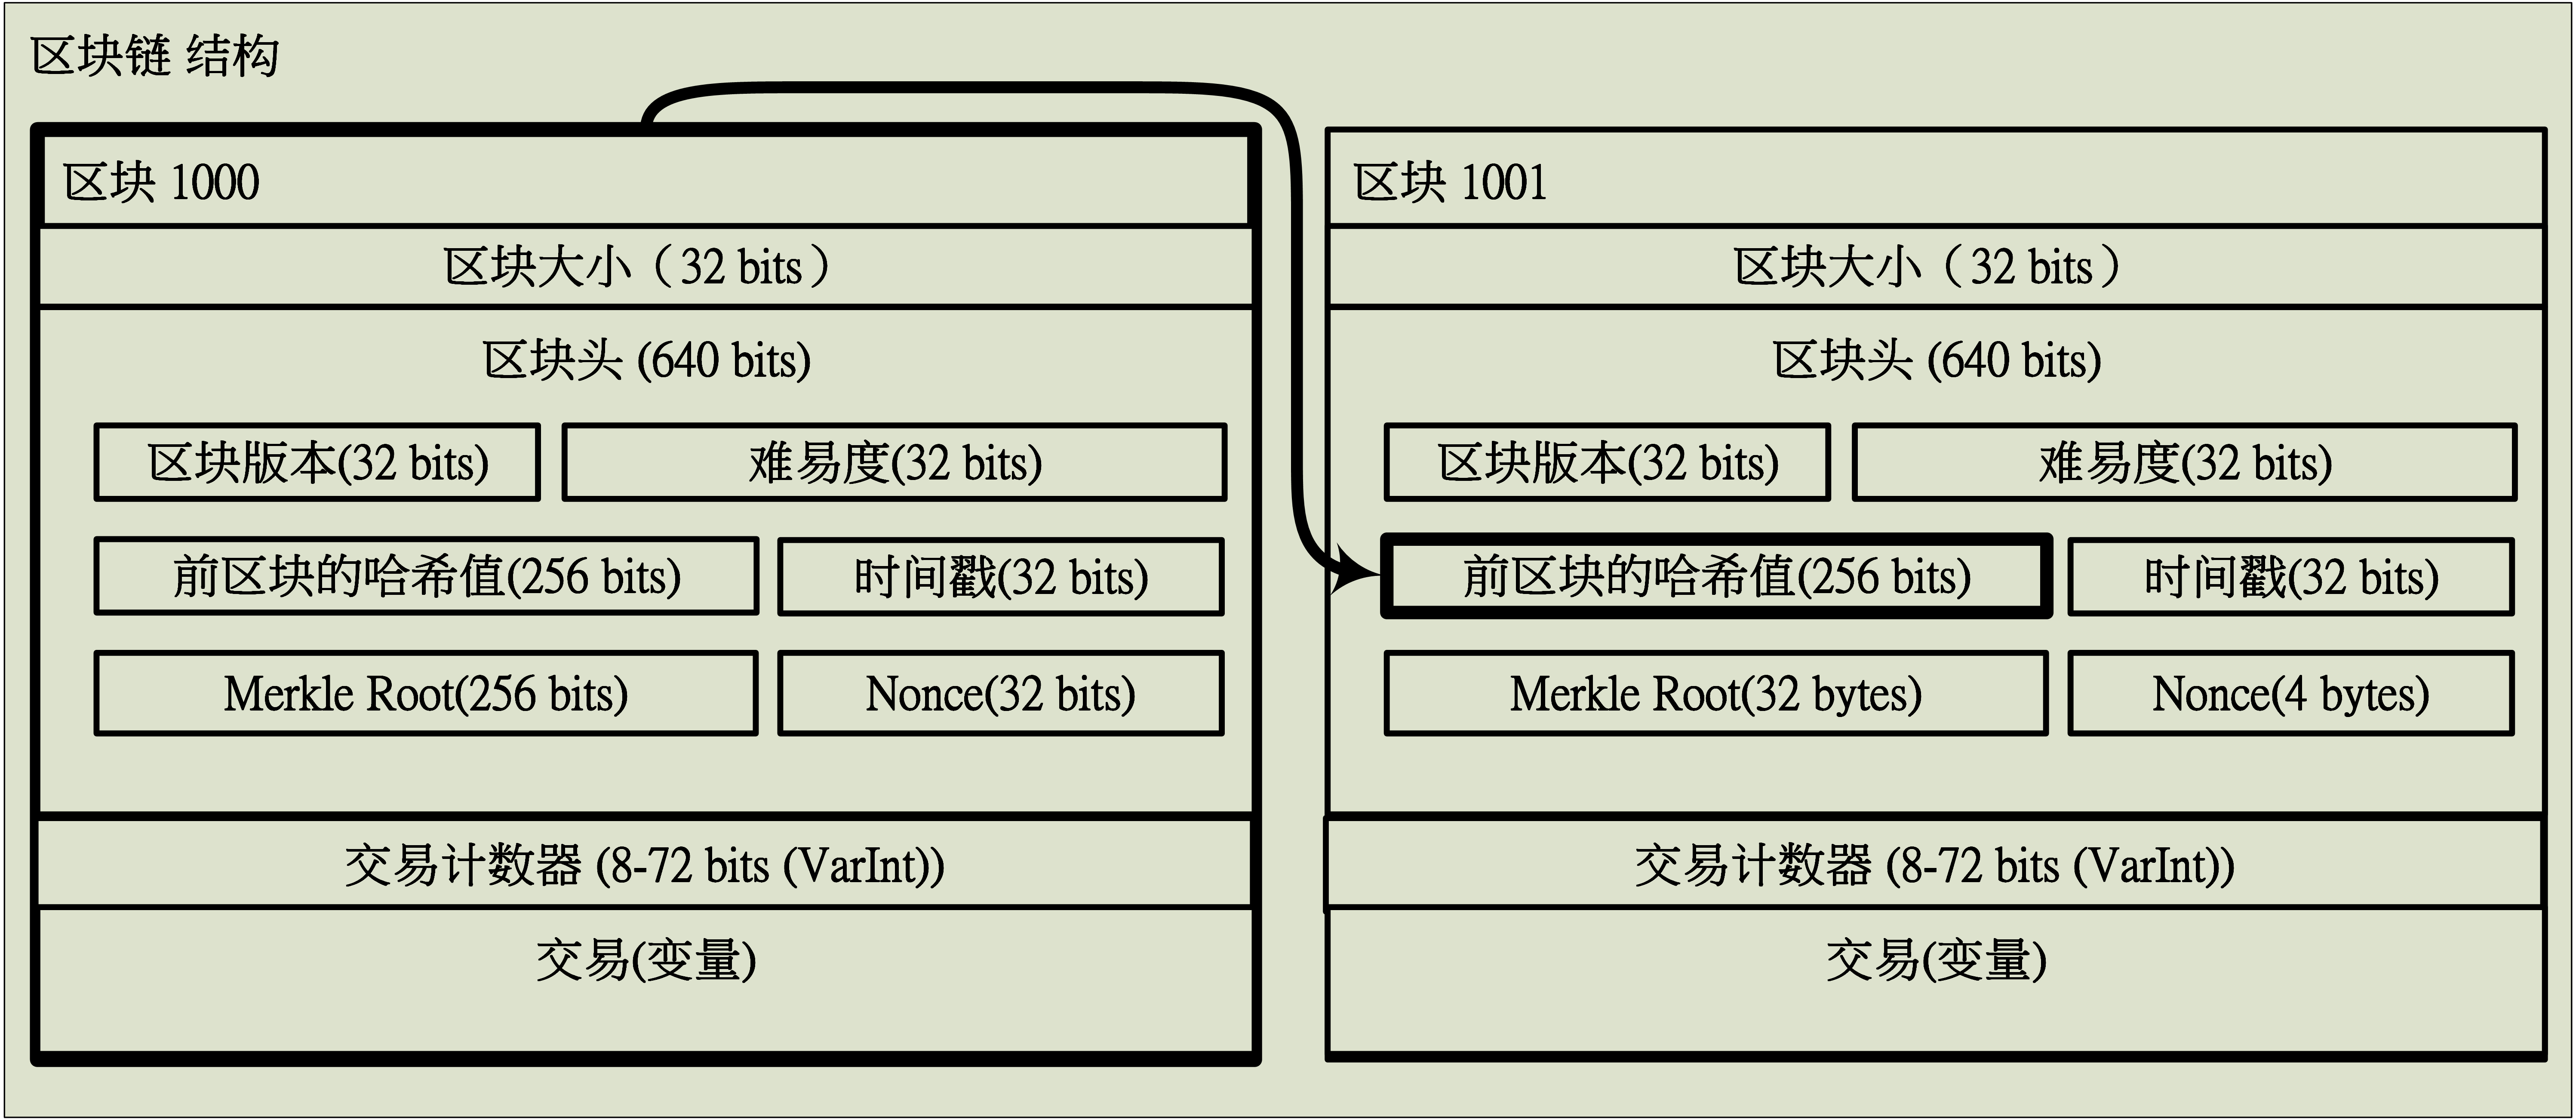
\includegraphics[width = 1\textwidth]{blockchain.png}
				\caption{比特幣區塊鏈結構圖}\label{blockchain}
			\end{figure}

				\begin{enumerate}
				\item 區塊版本(32 bits):該欄位存儲比特幣區塊鏈中的區塊版本。
				\item 前區塊的哈希值(256 bits):記錄前一個區塊的哈希值。 根據當前區塊的前一個區塊哈希值進而形成哈希指針,所有塊可以因為哈希指針連接在一起形成比特幣區塊鏈,不僅可以在區塊與區塊間建立虛擬鏈接,還可以使得區塊更難以被篡改。而通過新區塊不斷疊加在舊區塊過程,舊區塊的哈希值將繼續傳遞到最新的區塊。若區塊上面堆疊更多的區塊,促使的哈希值間接引用越多次,因此較早創建的區塊更難以修改。
				\item Merkle Root(256 bits):Merkle Root的生成方法是將當前區塊的所有交易為$n$個進行排序後,Merkle Root為Merkle Tree的樹根,交易為樹葉$n$個,將每個樹葉進行兩次SHA-256哈希算法取得哈希值得到$n$個哈希值,再將哈希值兩兩配對合併進行兩次SHA-256,得到$n*2^{-1}$個哈希值後,在$k$輪後會使得$n*2^{-k}=1$時,合併到只剩下一個哈希值,最後一個哈希值則為Merkle Root,如圖所示\ref{MerkleRoot},圖中的Hash()函數為雙重SHA-256,在區塊鏈中的Merkle Root可用於快速檢查當前區塊中所有存儲交易的正確性。

				\begin{figure}[htbp]
					\centering
					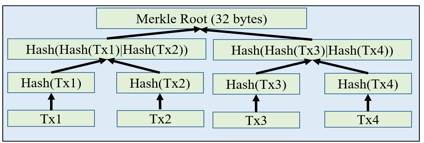
\includegraphics[width = 0.7\textwidth]{MerkleRoot.png}
					\caption{Merkle Tree示意圖}\label{MerkleRoot}
				\end{figure}

				\item 難易度(32 bits):難易度參數主要調控比特幣挖礦過程中採用工作量證明算法的變量,執得一提的是比特幣的難易度參數為動態調整。在過去的加密貨幣的設計中,有著因為沒有動態修改區塊難度,而導致區塊鏈生成速度太快,甚至導致區塊鏈系統崩潰。
				\item 時間戳(32 bits):以年、月、日、小時和秒的格式記錄區塊生成時間。
				\item Nonce(32 bits):Nonce記錄著礦工在進行挖礦時,必須要不斷的嘗試Nonce參數,直到符合難易度參數,才可以創建一個全新的比特幣區塊。該值為32 bits ,意為著礦工嘗試的組態空間為$2^{32}$個可能性。
				\end{enumerate}
				
		%區塊內容 交易手續費攻擊
			%\subsection{Block Data}
			%	\subsubsection{交易計數器 (4-36 bits)}
			%	\subsubsection{交易信息}

		%\section{工作量證明(Proof of Work)}
		\section{點對點網絡與加密貨幣安全}

		去中⼼化的加密貨幣系統給社會和傳統中⼼化的⾦融體系,以及政府帶來了很重⼤的衝擊,Satoshi Nakamoto建構了一個不需要中央銀行發行貨幣的貨幣系統,在比特幣的貨幣發行上全靠區塊鏈既定的算法。除了貨幣發行,也將交易記錄的帳本以明文的方式存儲在去中心化的區塊鏈中,以比特幣為例,現今完整的比特幣區塊鏈帳本已經高達180GB,這樣保存完整交易數據的計算機稱之為全節點,在比特幣去中心化的網絡中,如圖\ref{bitcoinfullnode}所示,截至2018年1月25比特幣網絡中全節點數量為10552個\supercite{bitcoinfullnode},全節點的數量決定了比特幣帳本的可靠度,倘若有著更多的全節點,會使得比特幣網絡堅不可摧,更難去修改歷史發生過的交易數據。

		\begin{figure}
			\centering
			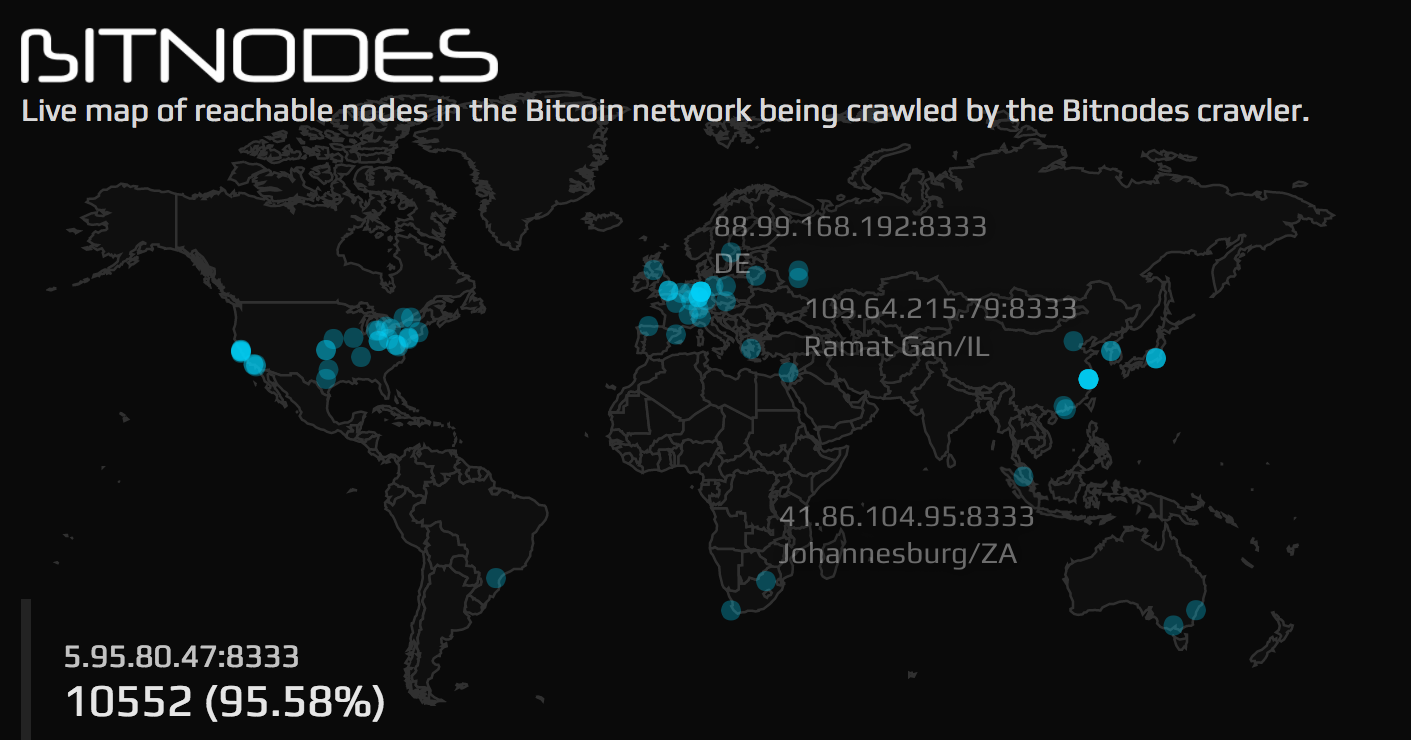
\includegraphics[width = .9\textwidth]{bitcoinfullnode.png}
			\caption{比特幣全節點分佈圖\supercite{bitcoinfullnode}}\label{bitcoinfullnode}
		\end{figure}

		% \section{山寨幣(Altcoin)簡介}

		% 	\subsection{萊特幣(Litecoin)}

		% 	\subsection{狗幣(Dogecoin)}

		% 	\subsection{域名幣(Namecoin)}

		% 	\subsection{以太坊(Etherum)}